\documentclass{article}
\usepackage{graphicx}
\usepackage{listings}

\begin{document}
\title{Homework 1}
\author{Lilong Jiang (jiang.573)}
\maketitle
\section{Problem 1}
Classifier: \\
1: if event is A \\
-1: if event is B \\
1: if event is C\\
Expected loss: 0.1 * 0.1 + 0.6 * 0.3 + 0.3 * 0.2 = 0.01 + 0.18 + 0.06 = 0.25 

\section{Problem 2}
Assume $P_1 = N(1, 2) = \frac{1}{2\sqrt{\pi}}e^\frac{-(x-1)^2}{4}$, $P_2 = N(5,1) = \frac{1}{\sqrt{2\pi}}e^\frac{-(x-5)^2}{2}$. If we solve $P_1 = P_2$, then we get 3.2219 and 14.7781 (we ignore this value since the probability after this is pretty low).\\
\begin{figure}
	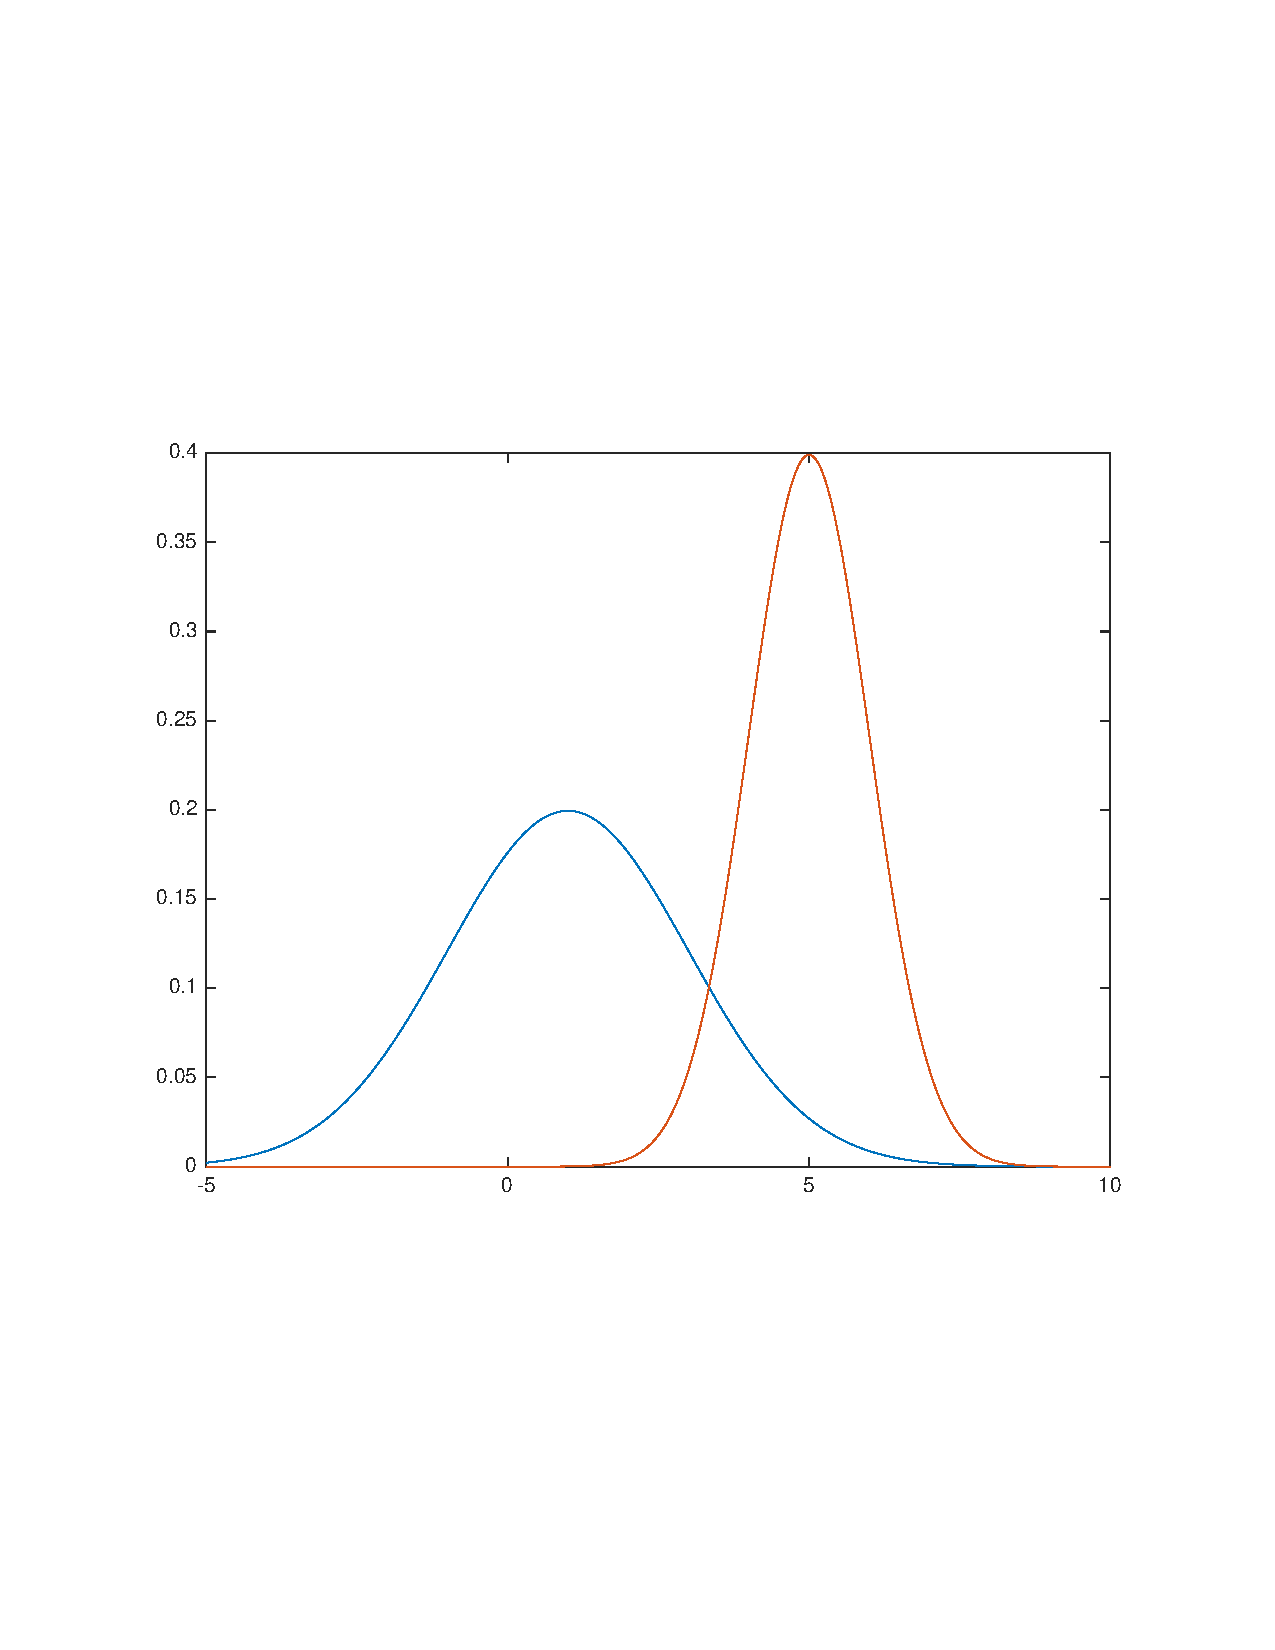
\includegraphics[width=\textwidth]{p2}
	\caption{Problem 2}
	\label{fig:p2}
\end{figure}
Figure~\ref{fig:p2} shows that the two normal distributions. \\
Classifier: \\
+1: if $x \leq 3.2219$ \\
-1: if $x > 3.2219$ \\
Bayes Risk: \\
$R = 0.6 * \int_{-\infty}^{3.2219}N(5, 1)dx + 0.4 * \int_{3.2219}^{\infty}N(1, 2)dx = 0.6* 0.0377 + 0.4 * 0.0581 = 0.0458$ \\

\section{Problem 3}
Expected Loss: \\
$E(loss(3NN)) = pC_3^0(1-p)^3 + pC_3^1p(1-p)^2 + (1-p)C_3^2p^2(1-p) + (1-p)C_3^3p^3 = p(1-p)^3 + 6p^2(1-p)^2 + (1-p)p^3$ \\
$E(loss(Bayes))) = 1 - p$ \\
$E(loss(3NN))-E(loss(Bayes)) \\ 
= p(1-p)^3 + 6p^2(1-p)^2 + (1-p)p^3 - (1 - p) \\
= (1-p)(p(1-p)^2 + 6p^2(1-p) + p^3 - 1) \\
= (1-p)(p^3 - 2p^2 + p + 6p^2 - 6p^3 + p^3) \\
= (1-p)(1-p)(4p-1) 
$ \\
The expected loss of 3NN is greater than Bayes optimal. \\
Since $p > 0.5$, $E(loss(3NN))-E(loss(Bayes)) > 0$. \\
Empirical Loss: \\
$E(emp(3NN)) = pC_2^0(1-p)^2 + (1-p)C_2^2p^2 = p(1-p)$ \\
$E(emp(3NN)) - E(loss(Bayes)) \\
= p(1-p) - (1-p)
= -(1-p)^2 < 0$
The empirical loss of 3NN is less than Bayes optimal.

\section{Problem 4}
\begin{lstlisting}
import numpy as np
import random
from scipy.spatial import distance
import matplotlib.pyplot as plt

class Point:
	def __init__(self, value, label):
		self.value = value
		self.label = label
		self.dist = float('inf')

def genData(num):
	data = []
	for i in xrange(num):
		coin = random.random()      #flip coin
		if coin > 0.5:
			value = np.random.multivariate_normal(mu1, I, 1)
			label = 1;
		else:
			value = np.random.multivariate_normal(mu2, I, 1)
			label = -1
		data.append(Point(value, label))
	return data

if __name__ == "__main__":
	errors1 = []
	errors2 = []
	ps = xrange(1, 102, 10)

	for p in ps:
		mu1 = np.zeros(p)
		mu2 = np.zeros(p)
		mu2[0] = 3
		I = np.identity(p)
		
	#training dataset
	trainPoints = genData(200)
	testPoints = genData(1000)
	
	#1NN
	errorNum = 0
	for testPoint in testPoints:
		dist = float("inf")
		classifyLabel = 0
		for trainPoint in trainPoints:
			curDist = distance.euclidean(testPoint.value, trainPoint.value)
			if curDist < dist:
				dist = curDist
				classifyLabel = trainPoint.label
		if classifyLabel != testPoint.label:
			errorNum += 1
			errors1.append(errorNum * 1.0 / 1000)
		
	#3NN      
	errorNum = 0
	for testPoint in testPoints:
		nearPoints = [Point(0, 0), Point(0, 0), Point(0, 0)]    #sorted by distance, maintain the nearest points so far
		classifyLabel = 0
		testLabel = testPoint.label
	
		for trainPoint in trainPoints:
			curDist = distance.euclidean(testPoint.value, trainPoint.value)
			if curDist < nearPoints[-1].dist: # the last one in the array has the largest distance
				trainPoint.dist = curDist
				nearPoints[-1] = trainPoint
				nearPoints = sorted(nearPoints, key=lambda point: point.dist)
				
		posNum = 0
		negNum = 0
		for nearPoint in nearPoints:
			if nearPoint.label > 0:
				posNum += 1
			else:
				negNum += 1
		if posNum > negNum:
			classifyLabel = 1
		else:
			classifyLabel = -1
		if classifyLabel != testLabel:
			errorNum += 1
			errors2.append(errorNum * 1.0 / 1000)
	print (errors1)
	print (errors2)
	fig, ax = plt.subplots()
	ax.plot(ps, errors1, 'ro', label='1NN')
	ax.plot(ps, errors2, 'g^', label='3NN')
	legend = ax.legend(loc='upper center', shadow=True)
	plt.show()
	plt.show()
\end{lstlisting}
\begin{figure}
	\centering
	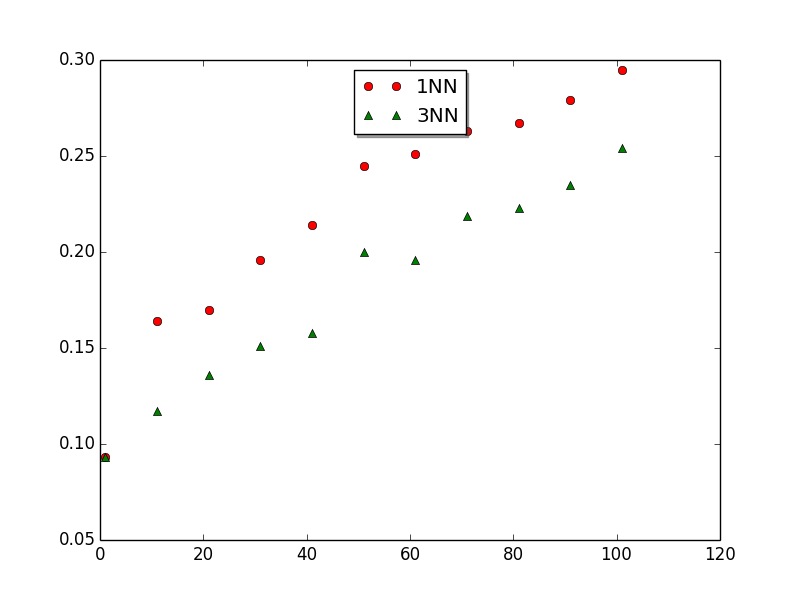
\includegraphics[width=\textwidth]{p4.png}
	\caption{Problem 4}
	\label{fig:p4}
\end{figure}
Figure~\ref{fig:p4} shows that with error increases with p. 

\section{Problem 5}
VC-dimension of the set of indicator functions of disks in $R^2$ is 3. Since for the following assignment with 3 points, it can't be shattered, shown in Figure~\ref{fig:p51}.
\begin{figure}
	\centering
	
\includegraphics[width=\textwidth]{p51}
	\caption{Problem 5}
	\label{fig:p51}
\end{figure}
For rectangle box, VC-dimension is 3, shown in Figure~\ref{fig:p51}. 
\end{document}